%%%%%%%%%%%%%%%%%%%%%%%%%%%%%%%%%%%%%%%%%
% Beamer Presentation
% LaTeX Template
% Version 1.0 (10/11/12)
%
% This template has been downloaded from:
% http://www.LaTeXTemplates.com
%
% License:
% CC BY-NC-SA 3.0 (http://creativecommons.org/licenses/by-nc-sa/3.0/)
%
%%%%%%%%%%%%%%%%%%%%%%%%%%%%%%%%%%%%%%%%%

%----------------------------------------------------------------------------------------
%	PACKAGES AND THEMES
%----------------------------------------------------------------------------------------

\documentclass{beamer}

\mode<presentation> {

% The Beamer class comes with a number of default slide themes
% which change the colors and layouts of slides. Below this is a list
% of all the themes, uncomment each in turn to see what they look like.


%\usetheme{Luebeck}
\usetheme{Madrid}
%\usetheme{Malmoe}
%\usetheme{Marburg}
}

% As well as themes, the Beamer class has a number of color themes
% for any slide theme. Uncomment each of these in turn to see how it
% changes the colors of your current slide theme.

%

%\setbeamertemplate{footline} % To remove the footer line in all slides uncomment this line
%\setbeamertemplate{footline}[page number] % To replace the footer line in all slides with a simple slide count uncomment this line

%\setbeamertemplate{navigation symbols}{} % To remove the navigation symbols from the bottom of all slides uncomment this line
\usepackage{xspace}
\usepackage{amsmath,mathrsfs,amscd}
\usepackage{subfig}
\usepackage{slashed}
\usepackage{graphicx} % Allows including images
\usepackage{booktabs} % Allows the use of \toprule, \midrule and \bottomrule in tables
\usepackage[compat=1.1.0]{tikz-feynman}
\newcommand\Tstrut{\rule{0pt}{3.0ex}}         % = `top' strut
\newcommand\Bstrut{\rule[-1.5ex]{0pt}{0pt}}   % = `bottom' strut
\newcommand{\ftapprox}{FT$_{\mathrm{approx}}$\xspace}
\newcommand{\nnloBP}{NNLO$_{\mathrm{B-proj}}$\xspace}
\newcommand{\nnloNI}{NNLO$_{\mathrm{NLO-i}}$\xspace}
\newcommand{\nnloFT}{NNLO$_{\mathrm{FTapprox}}$\xspace}
\newcommand{\nloFT}{NLO$_{\mathrm{FTapprox}}$\xspace}
\newcommand{\sqrtS}{\ensuremath{\sqrt{s}}}
\def\E#1{\times 10^{#1}}

%----------------------------------------------------------------------------------------
%	TITLE PAGE
%----------------------------------------------------------------------------------------

\title[tth]{Measure Higgs CP via tth Channel} % The short title appears at the bottom of every slide, the full title is only on the title page

\author{Ren-Qi Pan} % Your name
\institute[ZJU] % Your institution as it will appear on the bottom of every slide, may be shorthand to save space
{
Zhejiang Institute of Modern Physics\\ % Your institution for the title page
\medskip
\textit{renqipan@zju.edu.cn} % Your email address
}
\date{\today} % Date, can be changed to a custom date

\begin{document}

\begin{frame}
\titlepage % Print the title page as the first slide
\end{frame}

\begin{frame}
\frametitle{Overview} % Table of contents slide, comment this block out to remove it
\tableofcontents % Throughout your presentation, if you choose to use \section{} and \subsection{} commands, these will automatically be printed on this slide as an overview of your presentation
\end{frame}

%----------------------------------------------------------------------------------------
%	PRESENTATION SLIDES
%----------------------------------------------------------------------------------------

%------------------------------------------------
\begin{frame}
\frametitle{with or without btag}
\begin{figure}
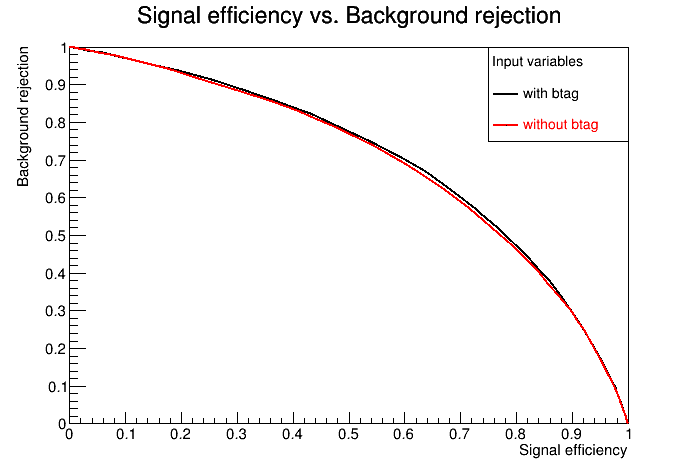
\includegraphics[scale=0.25]{./figures/ROC_Curve_btag.png}
\caption{compare the ROC curve between with and without btag.}
\end{figure}
\end{frame}


\begin{frame}
\frametitle{6 jets vs. 10 jets }
\begin{figure}
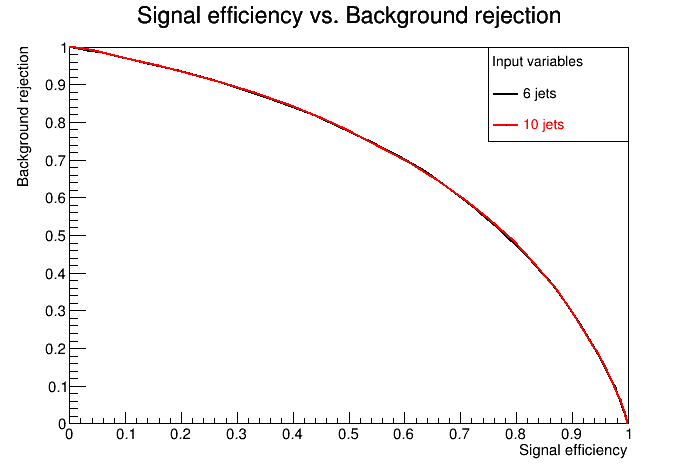
\includegraphics[scale=0.25]{./figures/ROC_Curve_jets.png}
\caption{compare the ROC curve between 6 jets and 10 jets.}
\end{figure}
\end{frame}

\begin{frame}
\frametitle{diphoton information vs. 2 photons information }
\begin{figure}
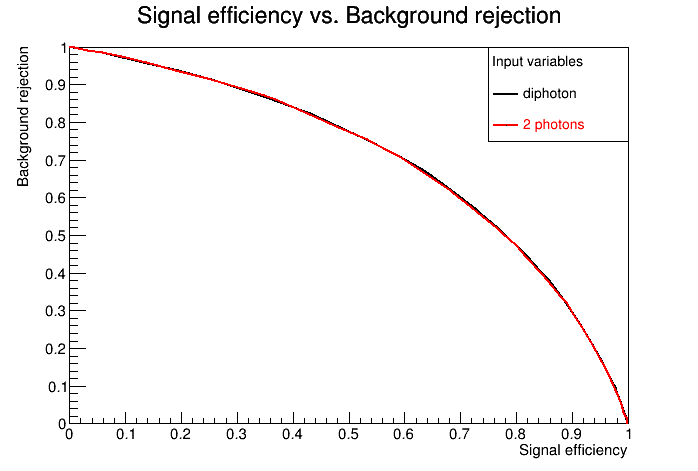
\includegraphics[scale=0.25]{./figures/ROC_Curve_photon.png}
\caption{compare the ROC curve between diphoton information and information of 2 photons.}
\end{figure}
\end{frame}

\begin{frame}
\frametitle{with or without diPhoMass }
\begin{figure}
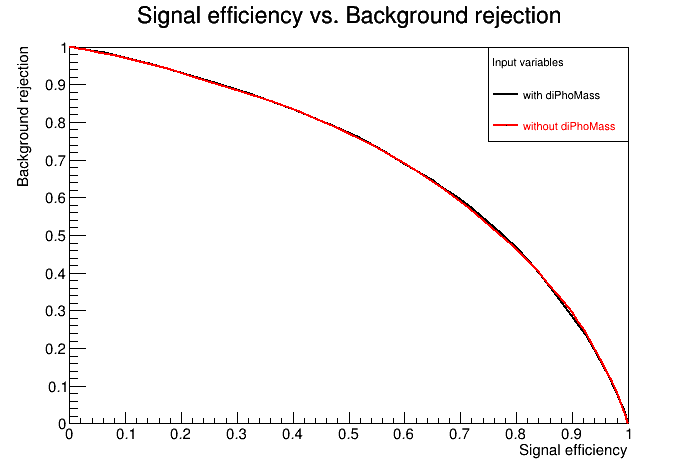
\includegraphics[scale=0.25]{./figures/ROC_Curve_diphomass.png}
\caption{compare the ROC curve between with and without diPhoMass.}
\end{figure}
\end{frame}

\begin{frame}
\frametitle{different input variables}
\begin{figure}
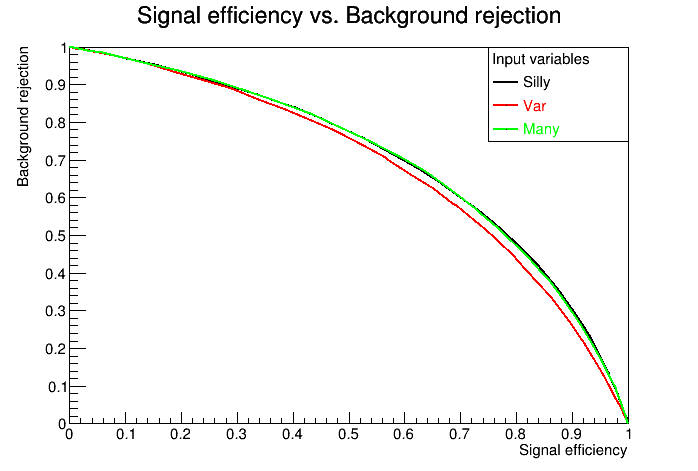
\includegraphics[scale=0.25]{./figures/ROC_Curve3.png}
\caption{compare the ROC curve between three different type of input variables.}
\end{figure}
\end{frame}


\begin{frame}
\frametitle{different tools}
\begin{figure}
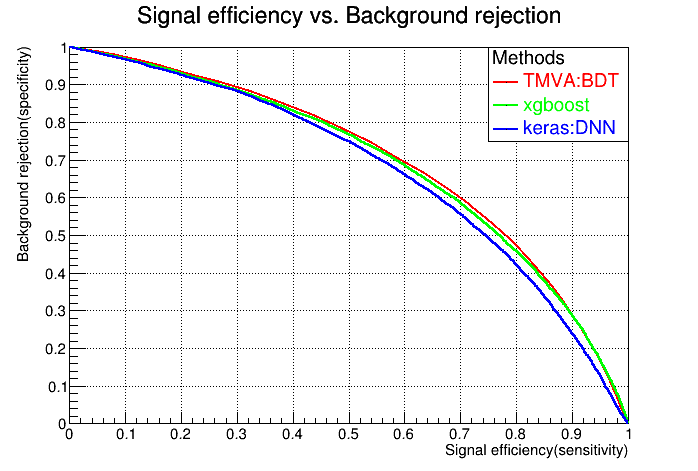
\includegraphics[scale=0.25]{./figures/tmva_xgboost.png}
\caption{compare the ROC curve between three different tools.}
\end{figure}
\end{frame}

\begin{frame}
\frametitle{Higgs boson decay}
\begin{figure}[H]
\centering
\subfloat[The branching ratios of Higgs boson near  $m_H = 125$ GeV]{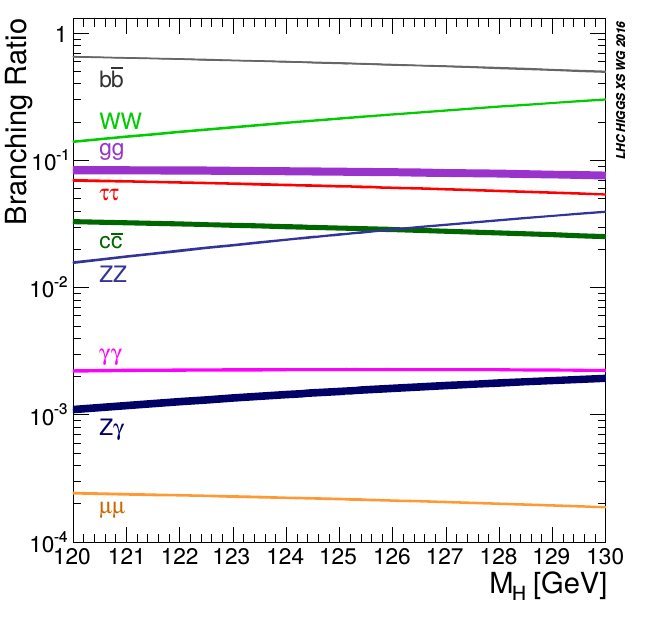
\includegraphics[width=0.45\textwidth]{./figures/higgs_ratio}} 
\subfloat[ The branching ratios of Higgs boson with $m_H = 125$ GeV]{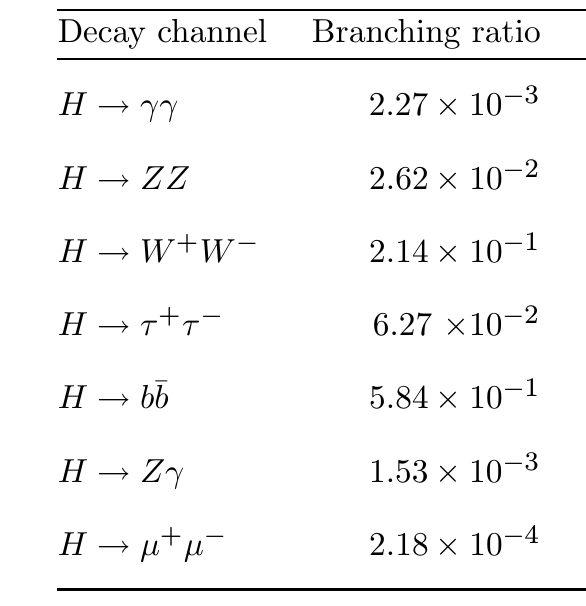
\includegraphics[width=0.41\textwidth]{./figures/higgs_ratio2}}
\caption{The main decay modes of Higgs Boson.Take from 	PDG-2016}
\end{figure}
\end{frame}






%------------------------------------------------

\begin{frame}
\Huge{\centerline{The End}}
\end{frame}

%----------------------------------------------------------------------------------------

\end{document} 